% Options for packages loaded elsewhere
\PassOptionsToPackage{unicode}{hyperref}
\PassOptionsToPackage{hyphens}{url}
\PassOptionsToPackage{dvipsnames,svgnames,x11names}{xcolor}
%
\documentclass[
  openany]{book}
\usepackage{amsmath,amssymb}
\usepackage{iftex}
\ifPDFTeX
  \usepackage[T1]{fontenc}
  \usepackage[utf8]{inputenc}
  \usepackage{textcomp} % provide euro and other symbols
\else % if luatex or xetex
  \usepackage{unicode-math} % this also loads fontspec
  \defaultfontfeatures{Scale=MatchLowercase}
  \defaultfontfeatures[\rmfamily]{Ligatures=TeX,Scale=1}
\fi
\usepackage{lmodern}
\ifPDFTeX\else
  % xetex/luatex font selection
\fi
% Use upquote if available, for straight quotes in verbatim environments
\IfFileExists{upquote.sty}{\usepackage{upquote}}{}
\IfFileExists{microtype.sty}{% use microtype if available
  \usepackage[]{microtype}
  \UseMicrotypeSet[protrusion]{basicmath} % disable protrusion for tt fonts
}{}
\makeatletter
\@ifundefined{KOMAClassName}{% if non-KOMA class
  \IfFileExists{parskip.sty}{%
    \usepackage{parskip}
  }{% else
    \setlength{\parindent}{0pt}
    \setlength{\parskip}{6pt plus 2pt minus 1pt}}
}{% if KOMA class
  \KOMAoptions{parskip=half}}
\makeatother
\usepackage{xcolor}
\usepackage[left=3cm,right=3cm,top=1cm,bottom=2cm]{geometry}
\usepackage{color}
\usepackage{fancyvrb}
\newcommand{\VerbBar}{|}
\newcommand{\VERB}{\Verb[commandchars=\\\{\}]}
\DefineVerbatimEnvironment{Highlighting}{Verbatim}{commandchars=\\\{\}}
% Add ',fontsize=\small' for more characters per line
\usepackage{framed}
\definecolor{shadecolor}{RGB}{248,248,248}
\newenvironment{Shaded}{\begin{snugshade}}{\end{snugshade}}
\newcommand{\AlertTok}[1]{\textcolor[rgb]{0.94,0.16,0.16}{#1}}
\newcommand{\AnnotationTok}[1]{\textcolor[rgb]{0.56,0.35,0.01}{\textbf{\textit{#1}}}}
\newcommand{\AttributeTok}[1]{\textcolor[rgb]{0.13,0.29,0.53}{#1}}
\newcommand{\BaseNTok}[1]{\textcolor[rgb]{0.00,0.00,0.81}{#1}}
\newcommand{\BuiltInTok}[1]{#1}
\newcommand{\CharTok}[1]{\textcolor[rgb]{0.31,0.60,0.02}{#1}}
\newcommand{\CommentTok}[1]{\textcolor[rgb]{0.56,0.35,0.01}{\textit{#1}}}
\newcommand{\CommentVarTok}[1]{\textcolor[rgb]{0.56,0.35,0.01}{\textbf{\textit{#1}}}}
\newcommand{\ConstantTok}[1]{\textcolor[rgb]{0.56,0.35,0.01}{#1}}
\newcommand{\ControlFlowTok}[1]{\textcolor[rgb]{0.13,0.29,0.53}{\textbf{#1}}}
\newcommand{\DataTypeTok}[1]{\textcolor[rgb]{0.13,0.29,0.53}{#1}}
\newcommand{\DecValTok}[1]{\textcolor[rgb]{0.00,0.00,0.81}{#1}}
\newcommand{\DocumentationTok}[1]{\textcolor[rgb]{0.56,0.35,0.01}{\textbf{\textit{#1}}}}
\newcommand{\ErrorTok}[1]{\textcolor[rgb]{0.64,0.00,0.00}{\textbf{#1}}}
\newcommand{\ExtensionTok}[1]{#1}
\newcommand{\FloatTok}[1]{\textcolor[rgb]{0.00,0.00,0.81}{#1}}
\newcommand{\FunctionTok}[1]{\textcolor[rgb]{0.13,0.29,0.53}{\textbf{#1}}}
\newcommand{\ImportTok}[1]{#1}
\newcommand{\InformationTok}[1]{\textcolor[rgb]{0.56,0.35,0.01}{\textbf{\textit{#1}}}}
\newcommand{\KeywordTok}[1]{\textcolor[rgb]{0.13,0.29,0.53}{\textbf{#1}}}
\newcommand{\NormalTok}[1]{#1}
\newcommand{\OperatorTok}[1]{\textcolor[rgb]{0.81,0.36,0.00}{\textbf{#1}}}
\newcommand{\OtherTok}[1]{\textcolor[rgb]{0.56,0.35,0.01}{#1}}
\newcommand{\PreprocessorTok}[1]{\textcolor[rgb]{0.56,0.35,0.01}{\textit{#1}}}
\newcommand{\RegionMarkerTok}[1]{#1}
\newcommand{\SpecialCharTok}[1]{\textcolor[rgb]{0.81,0.36,0.00}{\textbf{#1}}}
\newcommand{\SpecialStringTok}[1]{\textcolor[rgb]{0.31,0.60,0.02}{#1}}
\newcommand{\StringTok}[1]{\textcolor[rgb]{0.31,0.60,0.02}{#1}}
\newcommand{\VariableTok}[1]{\textcolor[rgb]{0.00,0.00,0.00}{#1}}
\newcommand{\VerbatimStringTok}[1]{\textcolor[rgb]{0.31,0.60,0.02}{#1}}
\newcommand{\WarningTok}[1]{\textcolor[rgb]{0.56,0.35,0.01}{\textbf{\textit{#1}}}}
\usepackage{longtable,booktabs,array}
\usepackage{calc} % for calculating minipage widths
% Correct order of tables after \paragraph or \subparagraph
\usepackage{etoolbox}
\makeatletter
\patchcmd\longtable{\par}{\if@noskipsec\mbox{}\fi\par}{}{}
\makeatother
% Allow footnotes in longtable head/foot
\IfFileExists{footnotehyper.sty}{\usepackage{footnotehyper}}{\usepackage{footnote}}
\makesavenoteenv{longtable}
\usepackage{graphicx}
\makeatletter
\def\maxwidth{\ifdim\Gin@nat@width>\linewidth\linewidth\else\Gin@nat@width\fi}
\def\maxheight{\ifdim\Gin@nat@height>\textheight\textheight\else\Gin@nat@height\fi}
\makeatother
% Scale images if necessary, so that they will not overflow the page
% margins by default, and it is still possible to overwrite the defaults
% using explicit options in \includegraphics[width, height, ...]{}
\setkeys{Gin}{width=\maxwidth,height=\maxheight,keepaspectratio}
% Set default figure placement to htbp
\makeatletter
\def\fps@figure{htbp}
\makeatother
\setlength{\emergencystretch}{3em} % prevent overfull lines
\providecommand{\tightlist}{%
  \setlength{\itemsep}{0pt}\setlength{\parskip}{0pt}}
\setcounter{secnumdepth}{5}
\usepackage{booktabs}
\ifLuaTeX
  \usepackage{selnolig}  % disable illegal ligatures
\fi
\usepackage[]{natbib}
\bibliographystyle{plainnat}
\IfFileExists{bookmark.sty}{\usepackage{bookmark}}{\usepackage{hyperref}}
\IfFileExists{xurl.sty}{\usepackage{xurl}}{} % add URL line breaks if available
\urlstyle{same}
\hypersetup{
  pdftitle={BayPass 2.3: tutoriel de génomique d'association adapté au séquençage en pool},
  pdfauthor={Jérôme OLIVARES},
  colorlinks=true,
  linkcolor={Maroon},
  filecolor={Maroon},
  citecolor={Blue},
  urlcolor={blue},
  pdfcreator={LaTeX via pandoc}}

\title{BayPass 2.3: tutoriel de génomique d'association adapté au séquençage en pool}
\author{Jérôme OLIVARES\footnote{INRAE, UR-1115 PSH, 228 route de l'aérodrome, 84914 Avignon, France}}
\date{2023-08-30}

\usepackage{amsthm}
\newtheorem{theorem}{Theorem}[chapter]
\newtheorem{lemma}{Lemma}[chapter]
\newtheorem{corollary}{Corollary}[chapter]
\newtheorem{proposition}{Proposition}[chapter]
\newtheorem{conjecture}{Conjecture}[chapter]
\theoremstyle{definition}
\newtheorem{definition}{Table}[chapter]
\theoremstyle{definition}
\newtheorem{example}{Script}[chapter]
\theoremstyle{definition}
\newtheorem{exercise}{Chunk}[chapter]
\theoremstyle{definition}
\newtheorem{hypothesis}{Hypothesis}[chapter]
\theoremstyle{remark}
\newtheorem*{remark}{Remark}
\newtheorem*{solution}{Solution}
\begin{document}
\maketitle

{
\hypersetup{linkcolor=}
\setcounter{tocdepth}{1}
\tableofcontents
}
\hypertarget{ruxe9sumuxe9}{%
\chapter*{Résumé}\label{ruxe9sumuxe9}}
\addcontentsline{toc}{chapter}{Résumé}

Ce tutoriel détaille d'une part la manière de générer les fichiers d'entrées du logiciel BayPass à partir de données de séquençage en pool, d'autre part le paramétrage optimal du logiciel BayPass et en fin propose une méthode d'exploreration des résultats d'analyses produits. Un pipeline d'analyse mixant des packages sous Rstudio et des lignes de commandes Linux, est décrit afin de guider pas à pas l'utilisateur tout au long du processus depuis les données brutes jusqu'à la liste finale de loci/variants candidats.
Ce tutoriel est à destination des étudiants et des bioinformaticiens débutants.

\hypertarget{mots-clefs}{%
\subsection*{mots clefs}\label{mots-clefs}}
\addcontentsline{toc}{subsection}{mots clefs}

Logiciel BayPass, séquençage en pool, GWAS, études d'associations pangénomiques, Rstudio.

\hypertarget{pruxe9requis}{%
\section*{prérequis}\label{pruxe9requis}}
\addcontentsline{toc}{section}{prérequis}

Les commandes décrites dans cet article ont été regroupées dans un fichier au format « R markdown » (Rmd) « Poolseq\_pipeline.Rmd » librement téléchargeable à l'adresse : \url{https://github.com/Jolivares-INRAE/Download}. Ce tutoriel est conçu pour décrire pas à pas les différentes étapes du fichier Rmd et permettre à l'utilisateur de les exécuter en parallèle.
L'utilisateur devra avoir une connaissance basique du logiciel Rstudio et être capable d'écrire et lancer des scripts sur un cluster de calcul.
Les commandes ont été rédigées sous Rstudio version 1.4.1106 couplé à R 64 bits version 4.0.5. avec toutes les librairies nécessaires à jour (Capture 1) et dans l'environnement bash/SLURM des clusters de calculs de la plateforme GenoToul de bioinformatique (GenoToul Bioinfo ). Dans le cas d'une utilisation dans un autre environnement logiciel, l'utilisateur devra probablement effectuer des adaptations du code.
Bien que l'essentiel des calculs de BayPass seront réalisés sur un cluster de calcul, certains de ses utilitaires seront utilisés en local sous Rstudio, la dernière version du logiciel sera donc téléchargée depuis l'adresse \url{https://forgemia.inra.fr/mathieu.gautier/baypass_public} et décompressée dans un répertoire local par l'utilisateur.
Dans tous les codes qui suivent l'expression «/../» sera à remplacer par les chemins personnels de l'utilisateur.
Le terme de chromosome sera utilisé en références aux appellations de contigs, scaffold, ou chromosomes qui correspondent aux séquences nucléotidiques du génome de référence, plus ou moins mature, qui sera utilisé.

\hypertarget{introduction}{%
\chapter*{Introduction}\label{introduction}}
\addcontentsline{toc}{chapter}{Introduction}

Dans un contexte agronomique actuel de réduction de l'utilisation des pesticides ou de réchauffement climatique, analyser et comprendre les bases génétiques de l'adaptation des organismes aux méthodes de luttes qui leurs sont opposées ou à l'évolution de leur environnement est un enjeu majeur des recherches de ces dernières années.

Les études d'associations pangénomiques (GWAS en anglais pour genome-wide association study) adossées aux techniques de séquençage haut débit (NGS) permettant le séquençage de génome complet, sont un outil de choix pour ce type d'analyse. L'étude au niveau populationnel demandant le séquençage d'un grand nombre d'individus, les couts d'analyses étaient initialement très élevés et ces études étaient souvent réservées aux organismes dit ``modèles'', humain en tête. Néanmoins il a été démontré depuis, que le séquençage en pool d'individus (poolseq) c'est-à-dire en mélangeant de manière équimolaire l'ADN d'un grand nombre d'individus (50 à 100) issus d'une même population permettait non seulement de réduire drastiquement les couts puisqu'on ne réalise qu'un seul séquençage mais aussi que la découverte des points de mutations (SNP) et l'estimation de leur fréquence allélique étaient souvent plus efficaces et précises \citep{futschik_next_2010}. Parmi les logiciels à même d'analyser ces fréquences alléliques on compte Baypass \citep{gautier_genome-wide_2015} qui évalue par une approche baysienne, la différenciation des SNP en liaison avec une covariable environnementale en tenant compte de la structure et de la parenté entre les populations en estimant la covariance (Ω) des fréquences alléliques. Baypass 2.3 a la particularité supplémentaire de pouvoir calculer un contraste des fréquences alléliques entre deux groupes de populations caractérisés par un caractère binaire, sensible ou résistant par exemple.

La documentation disponible de BayPass 2.3 décrit par le menu les algorithmes de fonctionnement et les différents paramètres du logiciel mais reste néanmoins, et assez logiquement, succincte sur les étapes en amont et en aval. A ma connaissance un seul tutoriel est disponible sur le web \citep{nielsen_pool-seq_2020} et décrit de manière plus détaillée la préparation des données brutes et l'analyse en mode « poolseq » de Baypass, mais il nécessite des bases quelque peu avancées de codage sous R et en environnement bash. Si les bio-informaticiens chevronnés ne rencontreront pas de difficultés particulières, il n'en va pas forcément de même pour bon nombre d'agents que les orientations des recherches associées à la baisse des coûts de séquençage ont aiguillé vers les voies de la génomique. Cet article a pour but de détailler les différentes étapes d'une analyse de type GWAS/poolseq avec le logiciel BayPass 2.3 et d'éclairer les points qui sont habituellement peu explicités car considérés comme évident.

\hypertarget{pruxe9sentation-du-logiciel-baypass-2.3}{%
\chapter*{Présentation du logiciel BayPass 2.3}\label{pruxe9sentation-du-logiciel-baypass-2.3}}
\addcontentsline{toc}{chapter}{Présentation du logiciel BayPass 2.3}

Le logiciel BayPass est un logiciel de génomique des populations qui vise principalement à l'identification de marqueurs génétiques soumis à la sélection et/ou associés à des covariables spécifiques à la population (variables environnementales, phénotypiques, quantitatives, catégorielles\ldots). Par une approche baysienne il évalue une \textbf{matrice Ω} de covariance des fréquences alléliques des populations résultant de leur histoire démographique. Deux manières d'estimer ces fréquences alléliques sont disponibles soit en se basant sur les génotypes référence/mutant des individus analysés soit, lorsque l'on active le « pool-seq mode », ces fréquences alléliques sont calculées en regard de la profondeur de séquençage (reads count) et pondérées par le nombre d'individus qui ont contribué à cette profondeur. C'est cette seconde approche que nous considérerons dans cet ouvrage.

BayPass propose 3 modèles statistiques d'analyse :

\hypertarget{le-core-model}{%
\subsubsection*{Le Core Model}\label{le-core-model}}
\addcontentsline{toc}{subsubsection}{Le Core Model}

C'est le modèle de base, il permet de calculer la matrice de covariance Ω et d'attribuer une statistique de différenciation XtX à chaque SNP, et ainsi de scanner le génome pour identifier les régions génomiques différenciées entre les populations.Le XtX est une statistique analogue au Fst mais tient compte de la co-évolution des populations grace à la matrice Ω.

\hypertarget{le-standard-model}{%
\subsubsection*{Le Standard Model}\label{le-standard-model}}
\addcontentsline{toc}{subsubsection}{Le Standard Model}

Ce modèle, permet, l'orsque l'on fournit une ou plusieurs covariables (environnementales, phénotypiques\ldots), de calculer un facteur de Bayes, ou Bayes factor en anglais, (BF) pour chaque marqueur génétique représentant la force d'association avec une covariable. C'est un modèle tout en un qui intègre le calcul des XtX et de la matrice Ω, il est adapté au faible nombre de population (\textless{} 15).

\hypertarget{lauxiliairy-model}{%
\subsubsection*{L'Auxiliairy Model}\label{lauxiliairy-model}}
\addcontentsline{toc}{subsubsection}{L'Auxiliairy Model}

Ce modèle a une approche différente dans le calcul de la statistique BF, sans entrer dans le détail il est plus adapté au grand nombre de population (\textgreater{} 15), En contrepartie il nécessite que l'on fournisse une matrice Ω déjà calculée par une analyse Core Model précédente, il recalcule alors les XtX et la statistique BF.

Ces covariables évoquées doivent être distribuées en gradient entre les populations (différence de température, d'altitude\ldots), en complément, dans le cas où la covariable étudiée serait purement qualitative ou binaire (sensible/résistant, gros/petit\ldots), les modèles Standard et Auxiliaire peuvent calculer une statistique C2 qui évalue le contraste de différence des fréquences alléliques de chaque marqueur entre 2 groupes de populations.

\hypertarget{pruxe9sentation-guxe9nuxe9rale-de-lanalyse}{%
\section*{Présentation générale de l'analyse :}\label{pruxe9sentation-guxe9nuxe9rale-de-lanalyse}}
\addcontentsline{toc}{section}{Présentation générale de l'analyse :}

La Figure \ref{fig:Fig1} est une vision simplifiée des différentes étapes nécessaire à l'analyses de données poolseq. Les étapes nécessittant une importante puissance de calcul comme le variant calling ou l'analyse BayPass se déroulent soit dans l'environnement Linux du cluster de calcul, les étapes de filtrage, manipulation de données et de résultats se font sur ordinateur local sous Rstudio.
La première étape part des fichiers d'alignement au format « \textbf{\emph{bam}} » de chaque population à analyser et consiste à effectuer une recherche de variants (variant calling) pour obtenir un fichier au format « *\textbf{\emph{vcf}} » regroupant tous les points de mutations ou SNP de toutes les populations qui sont autant de marqueurs génétiques à analyser. Ce fichier \textbf{\emph{vcf}} sert d'entrée au package « PoolFstat » \citep{gautier_f-statistics_2022} qui va permettre de filtrer les SNPs à analyser et générer les fichiers nécessaires au bon fonctionnement de BayPass mais aussi de faire une première analyse des Fst entre populations par exemple. Ces fichiers d'entrées pouvant contenir plusieurs millions de SNP, ils sont découpés en plusieurs dizaines de sous jeux de données (sub sampling) afin de réduire les temps de calculs. Une fois que BayPass a analysé tous les sous jeux de données, l'homogénéité des résultats entre eux est analysée sous Rstudio puis les résultats peuvent être regroupés, filtrés et analysés afin de déterminer les marqueurs génétiques et les régions chromosomiques d'intérêts qui seront visualisées par différents plots.

\begin{figure}
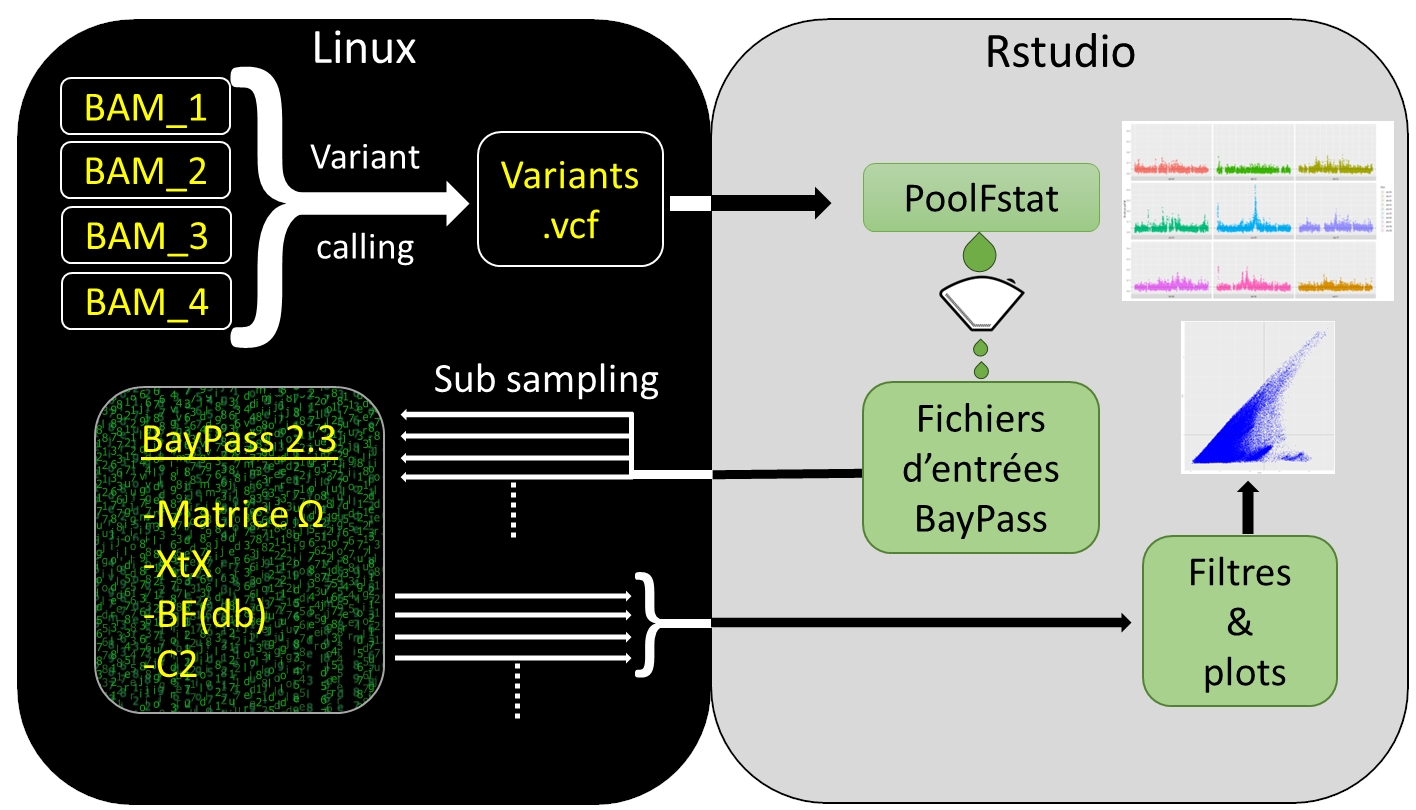
\includegraphics[width=19.67in]{images/Analyse2} \caption{Pipeline d'analyse BayPass}\label{fig:Fig1}
\end{figure}

Le pipeline d'analyse est décomposé en plusieurs étapes se déroulant soit en environnement Linux pour celles nécessitant une importante capacité de calcul, soit sous Rstudio pour le filtrage et l'analyse des résultats.

\hypertarget{donnuxe9es-brutes}{%
\chapter*{Données brutes}\label{donnuxe9es-brutes}}
\addcontentsline{toc}{chapter}{Données brutes}

\hypertarget{obtention-dun-fichier-poolseq.vcf}{%
\section*{Obtention d'un fichier Poolseq.vcf :}\label{obtention-dun-fichier-poolseq.vcf}}
\addcontentsline{toc}{section}{Obtention d'un fichier Poolseq.vcf :}

Les étapes de contrôle qualité et d'alignement des données de séquençage sont largement documentés par ailleurs, et ne serons donc pas documenter ici, et nous partirons directement des fichiers d'alignement \textbf{\emph{bam}}. La première étape consiste à regrouper les fichiers \textbf{\emph{bam}} de toutes les populations en un seul fichier puis à effectuer le variant calling avec un logiciel dédié compatible avec le séquençage en pool afin de conserver les informations de profondeur. Nous recommandons l'utilisation des Samtools \citep{li_sequence_2009} et de Varscan 2 \citep{koboldt_varscan_2012} avec une instruction pipe entre les deux pour éviter les fichiers intermédiaires et économiser l'espace de travail (Script \ref{exm:script1}). Les commandes sont effectuées avec les paramètres de base, sauf la p-value qui est montée à 0.5 pour être le moins stringent possible à ce stade. On peut découper le travail en plusieurs chromosomes pour réduire les temps de calculs.

\begin{example}
\protect\hypertarget{exm:script1}{}\label{exm:script1}{Exemple d'un script bash pour effectuer un variant calling}
\end{example}

Si l'on veut découper le travail en chromosomes, il est indispensable de travailler sur des fichiers bam correctement indexés et d'utiliser l'option -r/--region qui tire profit de cet index.

\begin{Shaded}
\begin{Highlighting}[]
\CommentTok{\#!/bin/bash}
\CommentTok{\#SBATCH {-}{-}array=1{-}29            \#création de l\textquotesingle{}array: un élément/indice par chromosome}

\ExtensionTok{module}\NormalTok{ load bioinfo/samtools/1.12}
\ExtensionTok{module}\NormalTok{ load bioinfo/VarScan/2.4.2}
\ExtensionTok{module}\NormalTok{ load bioinfo/bcftools/1.14}

\FunctionTok{ls}\NormalTok{ /My\_path/}\PreprocessorTok{*}\NormalTok{.bam }\OperatorTok{\textgreater{}}\NormalTok{ BamList.txt                                                }\CommentTok{\#liste tous les fichiers "bam" et leur chemin}
\FunctionTok{ls}\NormalTok{ /../}\PreprocessorTok{*}\NormalTok{.bam }\KeywordTok{|} \FunctionTok{sed} \AttributeTok{{-}r} \StringTok{\textquotesingle{}s/\^{}.+\textbackslash{}///\textquotesingle{}} \KeywordTok{|} \FunctionTok{sed} \AttributeTok{{-}r} \StringTok{\textquotesingle{}s/.bam//\textquotesingle{}} \OperatorTok{\textgreater{}}\NormalTok{ NameList.txt      }\CommentTok{\#extrait les noms des échatillons/populations}

\ExtensionTok{samtools}\NormalTok{ mpileup }\AttributeTok{{-}C}\NormalTok{ 50 }\AttributeTok{{-}d}\NormalTok{ 5000 }\AttributeTok{{-}q}\NormalTok{ 20 }\DataTypeTok{\textbackslash{}}
\NormalTok{{-}r chr}\VariableTok{$\{SLURM\_ARRAY\_TASK\_ID\}} \DataTypeTok{\textbackslash{} }                                           \CommentTok{\#attribut un chr à chaque indice de l\textquotesingle{}array : chr1, chr2 ...}
\ExtensionTok{{-}f}\NormalTok{ /../ref\_genome.fas }\AttributeTok{{-}b}\NormalTok{ /../BamList.txt }\KeywordTok{|} \DataTypeTok{\textbackslash{}}
\ExtensionTok{java} \AttributeTok{{-}Xmx2G} \AttributeTok{{-}jar} \VariableTok{$VARSCAN}\NormalTok{ mpileup2cns }\DataTypeTok{\textbackslash{}}
\NormalTok{{-}{-}variants }\AttributeTok{{-}{-}min{-}coverage}\NormalTok{ 10 }\DataTypeTok{\textbackslash{}}
\NormalTok{{-}{-}min{-}avg{-}qual 20 }\AttributeTok{{-}{-}min{-}var{-}freq}\NormalTok{ 0.05 }\DataTypeTok{\textbackslash{}}
\NormalTok{{-}{-}p{-}value 0.5 }\AttributeTok{{-}{-}output{-}vcf}\NormalTok{ 1 }\DataTypeTok{\textbackslash{}}
\NormalTok{{-}{-}vcf{-}sample{-}list NameList.txt }\OperatorTok{\textgreater{}}\NormalTok{ /../project\_chr}\VariableTok{$\{SLURM\_ARRAY\_TASK\_ID\}}\NormalTok{.vcf}

\ExtensionTok{bgzip}\NormalTok{ /../project\_chr}\VariableTok{$\{SLURM\_ARRAY\_TASK\_ID\}}\NormalTok{.vcf}
\ExtensionTok{bcftools}\NormalTok{ index /../project\_chr}\VariableTok{$\{SLURM\_ARRAY\_TASK\_ID\}}\NormalTok{.vcf}
\end{Highlighting}
\end{Shaded}

A l'issue du variant calling les fichiers \textbf{\emph{vcf}} des autosomes seront concaténés (Script \ref{exm:script2}), les chromosomes sexuels ayant une ségrégation, une histoire démographique et une ploïdie différente des autosomes il conviendra, lorsque cela est possible, de les analyser à part.

\begin{example}
\protect\hypertarget{exm:script2}{}\label{exm:script2}{Exemple d'un script bash pour concaténer des fichiers \textbf{\emph{vcf}}}
\end{example}

On peut utiliser les bcftools pour concaténer les fichier \textbf{\emph{vcf}}, la liste des fichiers à traiter est contenue dans une variable alimentée par une boucle ``for''.

\begin{Shaded}
\begin{Highlighting}[]
\CommentTok{\#!/bin/bash}
\ExtensionTok{module}\NormalTok{ load bioinfo/bcftools/1.14}
\VariableTok{my\_path}\OperatorTok{=}\StringTok{\textquotesingle{}/../\textquotesingle{}}

\CommentTok{\# une boucle "for" itére sur les numéros des autosomes de 2 à 28 et ajoute chaque fichier vcf et son chemin dans une variable}
\ControlFlowTok{for} \KeywordTok{((}\VariableTok{i}\OperatorTok{=}\DecValTok{2}\KeywordTok{;} \VariableTok{i}\OperatorTok{\textless{}=}\DecValTok{28}\KeywordTok{;} \VariableTok{i}\OperatorTok{++}\KeywordTok{))}
\ControlFlowTok{do}
    \VariableTok{files}\OperatorTok{+=}\StringTok{" }\VariableTok{$my\_path}\StringTok{/project\_chr}\VariableTok{$\{i\}}\StringTok{.vcf.gz"}  
\ControlFlowTok{done}

\CommentTok{\# bcftools concatène la liste des vcf contenu dans la variable $file}
\ExtensionTok{bcftools}\NormalTok{ concat }\VariableTok{$files} \AttributeTok{{-}O}\NormalTok{ z }\AttributeTok{{-}o} \VariableTok{$my\_path}\NormalTok{/project\_chr2{-}28.vcf.gz}
\end{Highlighting}
\end{Shaded}

\hypertarget{filtrage-des-donnuxe9es-brutes}{%
\section*{Filtrage des données brutes}\label{filtrage-des-donnuxe9es-brutes}}
\addcontentsline{toc}{section}{Filtrage des données brutes}

Le fichier \textbf{\emph{vcf}}, éventuellement compressé, est téléchargé sur un ordinateur local pour être analysé sous Rstudio.
Dans un premier temps il faut charger les packages nécessaires et définir les chemins des différents dossiers qui seront utilisés (Chunk \ref{exr:chunk1})

\begin{exercise}
\protect\hypertarget{exr:chunk1}{}\label{exr:chunk1}{Chargement des packages et chemins}
\end{exercise}

\begin{Shaded}
\begin{Highlighting}[]
\FunctionTok{library}\NormalTok{(poolfstat)      }\CommentTok{\#filtrage du vcf et création des fichiers d\textquotesingle{}entrées BayPass}
\FunctionTok{library}\NormalTok{(RColorBrewer)   }\CommentTok{\#gestion couleur des heatmaps}
\FunctionTok{library}\NormalTok{(mixOmics)       }\CommentTok{\#"cim" pour heatmap}
\FunctionTok{library}\NormalTok{(corrplot)       }\CommentTok{\#matrice de corrélation pour heat map}
\FunctionTok{library}\NormalTok{(VennDiagram)    }\CommentTok{\#création de diagramme de Venn}
\FunctionTok{library}\NormalTok{(nVennR)         }\CommentTok{\#extraction de données d\textquotesingle{}un diagramme de Venn}
\FunctionTok{library}\NormalTok{(tidyverse)      }\CommentTok{\#manipulation de données (dplyr) et plots (ggplot2)}

\CommentTok{\#définition des chemins de travail}
\NormalTok{path\_vcf }\OtherTok{\textless{}{-}} \StringTok{"/../vcf/"}
\NormalTok{path\_input }\OtherTok{\textless{}{-}} \StringTok{"/../Input/"}
\NormalTok{path\_out }\OtherTok{\textless{}{-}} \StringTok{"/../Output/"}
\NormalTok{path\_res }\OtherTok{\textless{}{-}} \StringTok{"/../Resultats/"}
\end{Highlighting}
\end{Shaded}

Le filtrage du \textbf{\emph{vcf}} et la sélection des SNPs à analyser ce fait à l'aide du package PoolFstat (Chunk \ref{exr:chunk2}). Dans un premier temps il faut renseigner les noms des populations dans un objet \textbf{\emph{pnames}} et les tailles haploïdes de chaque population dans un objet \textbf{\emph{psizes}}. Pour les organismes diploïdes, le nombre total de copies des autosomes sera deux fois le nombre d'individus dans le pool, pour les gonosomes Y ou W la ploïdie sera égale au nombre d'individus XY/ZW et pour les gonosomes X ou Z le calcul sera (nombre de XX/ZZ * 2) + (nombre de XY/ZW * 1).
La fonction \textbf{\emph{vcf2poodata}} va balayer le fichier \textbf{\emph{vcf}}, sélectionner les SNP bi-alléliques selon des critères définis par l'utilisateur et créer un objet \textbf{\emph{pooldata}}.

\begin{exercise}
\protect\hypertarget{exr:chunk2}{}\label{exr:chunk2}{Filtrage et sélection des SNPs}
\end{exercise}

Les options à renseigner sont:
min.rc = minimum de reads qu'un allèle doit avoir pour être retenu.
min.cov.per.pool = Si au moins un pool n'est pas couvert par au moins au moins min.cov.perpool reads, le SNP est rejeté.
max.cov.per.pool = Si au moins un pool est couvert par plus de que max.cov.perpool reads, le SNP est rejeté.
min.maf = fréquence allélique minimale autorisée pour l'allèle minoritaire pour qu'un SNP soit retenu.

\begin{Shaded}
\begin{Highlighting}[]
\CommentTok{\#Infos sur les pops}
\NormalTok{pnames }\OtherTok{\textless{}{-}} \FunctionTok{as.character}\NormalTok{(}\FunctionTok{c}\NormalTok{(}\StringTok{\textquotesingle{}pop01\textquotesingle{}}\NormalTok{, }\StringTok{\textquotesingle{}pop02\textquotesingle{}}\NormalTok{, }\StringTok{\textquotesingle{}pop03\textquotesingle{}}\NormalTok{, }\StringTok{\textquotesingle{}pop04\textquotesingle{}}\NormalTok{, }\StringTok{\textquotesingle{}pop05\textquotesingle{}}\NormalTok{, }\StringTok{\textquotesingle{}pop06\textquotesingle{}}\NormalTok{, }\StringTok{\textquotesingle{}pop07\textquotesingle{}}\NormalTok{, }\StringTok{\textquotesingle{}pop08\textquotesingle{}}\NormalTok{, }\StringTok{\textquotesingle{}pop09\textquotesingle{}}\NormalTok{, }\StringTok{\textquotesingle{}pop10\textquotesingle{}}\NormalTok{, }\StringTok{\textquotesingle{}pop11\textquotesingle{}}\NormalTok{, }\StringTok{\textquotesingle{}pop12\textquotesingle{}}\NormalTok{, }\StringTok{\textquotesingle{}pop13\textquotesingle{}}\NormalTok{))}
\NormalTok{psizes\_A }\OtherTok{\textless{}{-}} \FunctionTok{as.numeric}\NormalTok{(}\FunctionTok{c}\NormalTok{(}\StringTok{\textquotesingle{}150\textquotesingle{}}\NormalTok{, }\StringTok{\textquotesingle{}180\textquotesingle{}}\NormalTok{, }\StringTok{\textquotesingle{}24\textquotesingle{}}\NormalTok{, }\StringTok{\textquotesingle{}114\textquotesingle{}}\NormalTok{, }\StringTok{\textquotesingle{}180\textquotesingle{}}\NormalTok{, }\StringTok{\textquotesingle{}44\textquotesingle{}}\NormalTok{,}\StringTok{\textquotesingle{}180\textquotesingle{}}\NormalTok{, }\StringTok{\textquotesingle{}160\textquotesingle{}}\NormalTok{, }\StringTok{\textquotesingle{}200\textquotesingle{}}\NormalTok{, }\StringTok{\textquotesingle{}74\textquotesingle{}}\NormalTok{, }\StringTok{\textquotesingle{}80\textquotesingle{}}\NormalTok{, }\StringTok{\textquotesingle{}52\textquotesingle{}}\NormalTok{, }\StringTok{\textquotesingle{}72\textquotesingle{}}\NormalTok{))   }\CommentTok{\#ploydie autosome}
\NormalTok{psizes\_X }\OtherTok{\textless{}{-}} \FunctionTok{as.numeric}\NormalTok{(}\FunctionTok{c}\NormalTok{(}\StringTok{\textquotesingle{}120\textquotesingle{}}\NormalTok{, }\StringTok{\textquotesingle{}135\textquotesingle{}}\NormalTok{, }\StringTok{\textquotesingle{}16\textquotesingle{}}\NormalTok{, }\StringTok{\textquotesingle{}86\textquotesingle{}}\NormalTok{, }\StringTok{\textquotesingle{}135\textquotesingle{}}\NormalTok{, }\StringTok{\textquotesingle{}30\textquotesingle{}}\NormalTok{,}\StringTok{\textquotesingle{}135\textquotesingle{}}\NormalTok{, }\StringTok{\textquotesingle{}120\textquotesingle{}}\NormalTok{, }\StringTok{\textquotesingle{}150\textquotesingle{}}\NormalTok{, }\StringTok{\textquotesingle{}60\textquotesingle{}}\NormalTok{, }\StringTok{\textquotesingle{}63\textquotesingle{}}\NormalTok{, }\StringTok{\textquotesingle{}42\textquotesingle{}}\NormalTok{, }\StringTok{\textquotesingle{}53\textquotesingle{}}\NormalTok{))    }\CommentTok{\#ploydie X/Z}
\NormalTok{psizes\_Y }\OtherTok{\textless{}{-}} \FunctionTok{as.numeric}\NormalTok{(}\FunctionTok{c}\NormalTok{(}\StringTok{\textquotesingle{}30\textquotesingle{}}\NormalTok{, }\StringTok{\textquotesingle{}45\textquotesingle{}}\NormalTok{, }\StringTok{\textquotesingle{}8\textquotesingle{}}\NormalTok{, }\StringTok{\textquotesingle{}28\textquotesingle{}}\NormalTok{, }\StringTok{\textquotesingle{}45\textquotesingle{}}\NormalTok{, }\StringTok{\textquotesingle{}14\textquotesingle{}}\NormalTok{,}\StringTok{\textquotesingle{}45\textquotesingle{}}\NormalTok{, }\StringTok{\textquotesingle{}40\textquotesingle{}}\NormalTok{, }\StringTok{\textquotesingle{}50\textquotesingle{}}\NormalTok{, }\StringTok{\textquotesingle{}14\textquotesingle{}}\NormalTok{, }\StringTok{\textquotesingle{}17\textquotesingle{}}\NormalTok{, }\StringTok{\textquotesingle{}10\textquotesingle{}}\NormalTok{, }\StringTok{\textquotesingle{}19\textquotesingle{}}\NormalTok{))           }\CommentTok{\#ploydie Y/W}
\CommentTok{\#conversion du .vcf}
\NormalTok{pooldata }\OtherTok{\textless{}{-}} \FunctionTok{vcf2pooldata}\NormalTok{(}\AttributeTok{vcf.file =} \FunctionTok{paste}\NormalTok{(path\_vcf, }\StringTok{"project\_chr2{-}28.vcf.gz"}\NormalTok{, }\AttributeTok{sep=}\StringTok{""}\NormalTok{), }\AttributeTok{poolsizes =}\NormalTok{ psizes\_A, }\AttributeTok{poolnames =}\NormalTok{ pnames, }\AttributeTok{min.cov.per.pool =} \DecValTok{4}\NormalTok{, }\AttributeTok{min.rc =} \DecValTok{2}\NormalTok{, }\AttributeTok{max.cov.per.pool =} \FloatTok{1e+06}\NormalTok{, }\AttributeTok{min.maf =} \FloatTok{0.05}\NormalTok{, }\AttributeTok{remove.indels =} \ConstantTok{FALSE}\NormalTok{, }\AttributeTok{nlines.per.readblock =} \FloatTok{1e+06}\NormalTok{)}
\CommentTok{\#élimine le 1\% supérieur considéré comme trop fortement couvert (région très dupliquée, biais de séquençage...)}
\NormalTok{pooldata}\OtherTok{\textless{}{-}}\FunctionTok{pooldata.subset}\NormalTok{(pooldata, }\AttributeTok{cov.qthres.per.pool =} \FunctionTok{c}\NormalTok{(}\DecValTok{0}\NormalTok{,}\FloatTok{0.99}\NormalTok{))}
\end{Highlighting}
\end{Shaded}

A ce stade cet objet \textbf{\emph{pooldata}} peut être utilisé pour calculer diverses statistiques couremment utilisées dans les études de génomique des populations, un exemple d'estimation de la structure génétique des populations déduite des Fst est donné en \protect\hyperlink{An1}{Annexe 1}

\hypertarget{conversion-du-pooldata-en-fichiers-dentruxe9es-pour-baypass}{%
\chapter*{Conversion du pooldata en fichiers d'entrées pour BayPass}\label{conversion-du-pooldata-en-fichiers-dentruxe9es-pour-baypass}}
\addcontentsline{toc}{chapter}{Conversion du pooldata en fichiers d'entrées pour BayPass}

La fonction \textbf{\emph{pooldata2genobaypass}} (Chunk \ref{exr:chunk3}) convertit l'ogbjet \textbf{\emph{pooldata}} en fichier d'entrée pour BayPass:

\begin{exercise}
\protect\hypertarget{exr:chunk3}{}\label{exr:chunk3}{Création des fichiers input de BayPass}
\end{exercise}

\begin{Shaded}
\begin{Highlighting}[]
\FunctionTok{pooldata2genobaypass}\NormalTok{(pooldata, }\AttributeTok{writing.dir =}\NormalTok{ path\_input, }\AttributeTok{subsamplesize =} \SpecialCharTok{{-}}\DecValTok{1}\NormalTok{, }\AttributeTok{subsamplingmethod =} \StringTok{"thinning"}\NormalTok{)}
\end{Highlighting}
\end{Shaded}

On récupère dans le répertoire \textbf{\emph{path\_input}} trois fichiers: un fichier ``\textbf{\emph{genobaypass}}'' qui contient les données filtrées de génotypage, un fichier ``\textbf{\emph{snpdet}}'' qui contient la liste des positions correspondantes et un fichier ``\textbf{\emph{poolsize}}'', qui est une copie de l'objet \textbf{\emph{psizes}}.

\hypertarget{design-de-lanalyse-baypass}{%
\section*{Design de l'analyse BayPass}\label{design-de-lanalyse-baypass}}
\addcontentsline{toc}{section}{Design de l'analyse BayPass}

Deux fichiers de paramétrages au format texte/tabulation peuvent être créés en fonction de l'analyse envisagé:
Le premier fichier ``\textbf{\emph{ecotype}}'' (Table \ref{def:table1}) identifie les covariables quantitatives écologiques de chaque population, avec une covariable par ligne et autant de lignes que de covariables à analyser. Seules sont acceptées les valeurs numériques graduées (taille, poids, mortalité \ldots).

\begin{definition}
\protect\hypertarget{def:table1}{}\label{def:table1}{Example de constitution d'un fichier \textbf{\emph{ecotype}}}
\end{definition}

Chaque ligne correspond à une covariable quantitative, chaque colonne correspond à une population.

25

48.5

96.2

17

15.3

\ldots{}

4.75

0.53

0.27

-0.86

-0.61

\ldots{}

43.90

44.37

44.29

47.36

47.86

\ldots{}

Le deuxième fichier \textbf{\emph{contraste}} (Table \ref{def:table2})contient les covariables qualitatives (petit, chaud, resistant\ldots), il permet d'identifier l'appartenance de chaque population à un groupe qualitatif soit référence (-1), un groupe candidat (1) ou aucun des deux groupes (0). Une ligne par combinaison de contraste.

\begin{definition}
\protect\hypertarget{def:table2}{}\label{def:table2}{Example de constitution d'un fichier \textbf{\emph{contraste}}}
\end{definition}

Chaque ligne correspond à une analyse binaire de comparaison des fréquences alléliques de 2 groupes de population.
Sur la ligne 1 le groupe composé des population 1 et 2 est comparé au groupe des populations 3,4 et 5.
Sur la ligne 2 le groupe composé des population 1 et 2 est comparé au groupe des populations 4 et 5, la population 3 est exclue de l'analyse.
Etc\ldots{}

1

1

-1

-1

-1

\ldots{}

1

1

0

-1

-1

\ldots{}

0

1

-1

-1

0

\ldots{}

Ces fichiers seront aussi transférés sur le cluster de calcul.

IMPORTANT : Les analyses BayPass sont relativement longues (plusieurs heures) mais l'analyses conjointes de plusieurs covariables a un impact relativement faible sur le temps de calcul final, dès lors il est très rentable de multiplier les analyses de covariables en ajoutant autant de lignes que nécessaires dans ces fichiers de paramétrages plutôt que de relancer une analyse complète pour chacune d'entre elles.

\hypertarget{subsampling}{%
\section*{Subsampling}\label{subsampling}}
\addcontentsline{toc}{section}{Subsampling}

Copier les fichiers \textbf{\emph{genobaypass, snpdet, poolsize, contraste, ecotype}} sur le cluster de calcul.
La découpe en sous jeux de données des fichier genobaypass et snpdet se fait sous Bash avec une commande sed par exemple (Script \ref{exm:script3}).

\begin{example}
\protect\hypertarget{exm:script3}{}\label{exm:script3}{Exemple d'une commande de subsampling.}
\end{example}

La commande \textbf{\emph{sed}} prélève une ligne toutes les 100 et les copies dans un fichier \textbf{\emph{.sub}} et s'exécute 100 fois pour ballayer tous le fichier initial et créer ainsi 100 fichiers de sous-jeux de données.

\begin{Shaded}
\begin{Highlighting}[]
\ControlFlowTok{for}\NormalTok{ i }\KeywordTok{in} \DataTypeTok{\{}\DecValTok{1}\DataTypeTok{..}\DecValTok{100}\DataTypeTok{\}}\KeywordTok{;} \ControlFlowTok{do} \FunctionTok{sed} \AttributeTok{{-}n} \StringTok{"}\VariableTok{$i}\StringTok{\textasciitilde{}100p"}\NormalTok{ genobaypass }\OperatorTok{\textgreater{}}\NormalTok{ genobaypass.sub}\VariableTok{$i}\KeywordTok{;} \FunctionTok{sed} \AttributeTok{{-}n} \StringTok{"}\VariableTok{$i}\StringTok{\textasciitilde{}100p"}\NormalTok{ snpdet }\OperatorTok{\textgreater{}}\NormalTok{ snpdet.sub}\VariableTok{$i}\KeywordTok{;} \ControlFlowTok{done}
\end{Highlighting}
\end{Shaded}

Le nombre de fichiers \textbf{\emph{.sub}} à créer dépend du nombre total de SNP à analyser, une taille finale de 80 000 à 120 000 SNPs par fichier de sous-jeux de données est un bon compromis entre qualité d'analyse et temps de calcul.

\hypertarget{baypass-lanalyse-poolseq}{%
\chapter*{Baypass : l'analyse poolseq}\label{baypass-lanalyse-poolseq}}
\addcontentsline{toc}{chapter}{Baypass : l'analyse poolseq}

La commande est la même pour les différents modèles employés par BayPass (Script \ref{exm:script4}), ce sont les fichiers optionnels qui définissent le modèle :
l'option poolsize active le mode Pool-Seq, pour le core model, seuls les fichiers genobaypass et snpdet sont nécessaires, on peut néanmoins faire une analyse de la statistique de contraste C2 avec le fichier de covariable qualitative \textbf{\emph{contraste}}.
Le modèle standard est activé par l'option \textbf{\emph{-efile}}, le fichier de covariable quantitative \textbf{\emph{ecotype}}.

Il est recommandé dans le cadre d'une analyse Pool-Seq d'utiliser et fixer le paramètre -d0yij à 1/5e de la valeur la plus faible du poolsize. (voir page 22 et 39 du manuel de BayPass).
Tous les fichiers de résultats cibleront le dossier dans lequel se trouve le script.

\begin{example}
\protect\hypertarget{exm:script4}{}\label{exm:script4}{Exemple d'un script bash pour lancer une analyse BayPass}
\end{example}

Les sous-jeux de données sont analysés en parallèle

\begin{Shaded}
\begin{Highlighting}[]
\CommentTok{\#!/bin/bash}
\CommentTok{\#SBATCH {-}{-}array=0{-}99        \#création de l\textquotesingle{}array: un élément/indice par job prévu (indice base 0)}
\CommentTok{\#SBATCH {-}{-}cpus{-}per{-}task=2   \#nbr de core par job}
\CommentTok{\#SBATCH {-}{-}mem{-}per{-}cpu=2G    \#mémoire partagée par tous les cores}

\ExtensionTok{module}\NormalTok{ purge}
\ExtensionTok{module}\NormalTok{ load statistics/R/4.2.2}
\ExtensionTok{module}\NormalTok{ load bioinfo/BayPass/2.4}
\ExtensionTok{module}\NormalTok{ load compilers/intel/2023.0.0    }\CommentTok{\#pour i\_baypass}
\CommentTok{\#module load mpi/openmpi/4.1.4}
\CommentTok{\#module load compilers/gcc/12.2.0       \#pour g\_baypass}


\CommentTok{\#définition du chemin ciblant les fichiers genobaypass et snpdet}
\VariableTok{my\_path}\OperatorTok{=}\StringTok{\textquotesingle{}/../Input/\textquotesingle{}}
\VariableTok{FILES\_R1}\OperatorTok{=}\VariableTok{($(}\FunctionTok{ls} \VariableTok{$my\_path}\NormalTok{/genobaypass.sub}\PreprocessorTok{*} \KeywordTok{|} \FunctionTok{sed} \AttributeTok{{-}r} \StringTok{\textquotesingle{}s/\^{}.+\textbackslash{}///\textquotesingle{}}\VariableTok{))}
\VariableTok{INPUT\_F1}\OperatorTok{=}\VariableTok{$\{FILES\_R1}\OperatorTok{[}\VariableTok{$SLURM\_ARRAY\_TASK\_ID}\OperatorTok{]}\VariableTok{\}}
\VariableTok{OUTPUT}\OperatorTok{=}\VariableTok{$\{FILES\_R1}\OperatorTok{[}\VariableTok{$SLURM\_ARRAY\_TASK\_ID}\OperatorTok{]/}\SpecialStringTok{genobaypass}\OperatorTok{/}\NormalTok{project.output}\VariableTok{\}}

\ExtensionTok{i\_baypass} \DataTypeTok{\textbackslash{}}
\NormalTok{{-}gfile }\VariableTok{$my\_path}\NormalTok{/}\VariableTok{$INPUT\_F1} \DataTypeTok{\textbackslash{} }                 \CommentTok{\#fichiers genobaypass.sub*}
\ExtensionTok{{-}poolsizefile} \VariableTok{$my\_path}\NormalTok{/poolsize }\DataTypeTok{\textbackslash{} }           \CommentTok{\#active le mode poolseq}
\ExtensionTok{{-}d0yij}\NormalTok{ 40 }\DataTypeTok{\textbackslash{} }                              \CommentTok{\#1/5e de la valeur la plus faible du poolsize}
\ExtensionTok{{-}seed}\NormalTok{ 5001 }\DataTypeTok{\textbackslash{}}
\NormalTok{{-}nthreads 2 }\DataTypeTok{\textbackslash{}}
\NormalTok{{-}outprefix }\VariableTok{$OUTPUT} \DataTypeTok{\textbackslash{}}
\end{Highlighting}
\end{Shaded}

Pour le modèle standard, il faut rajouter au script précédent le fichier contenant les covariables quantitatives:

\begin{Shaded}
\begin{Highlighting}[]
\ExtensionTok{{-}efile} \VariableTok{$my\_path}\NormalTok{/ecotype }\DataTypeTok{\textbackslash{} }                   \CommentTok{\#calcul des Bayes Factors: modèle standard \& auxiliaire}
\ExtensionTok{{-}contrastfile} \VariableTok{$my\_path}\NormalTok{/contrast }\DataTypeTok{\textbackslash{} }           \CommentTok{\#calcul du contraste C2: modèle core, standard \& auxiliaire}
\end{Highlighting}
\end{Shaded}

Pour le modèle auxiliaire, il faut rajouter au script précédent en plus des fichiers covariables:

\begin{Shaded}
\begin{Highlighting}[]
\ExtensionTok{{-}auxmodel} \DataTypeTok{\textbackslash{} }                              \CommentTok{\#active le modèle auxiliaire}
\ExtensionTok{{-}omegafile} \VariableTok{$my\_path}\NormalTok{/omega.mat }\DataTypeTok{\textbackslash{} }          \CommentTok{\#matrice Ω modèle standard (optionnel) \& auxiliaire (obligatoire)}
\ExtensionTok{{-}auxPbetaprior}\NormalTok{ 0.02 1.98                  }\CommentTok{\#ajuste le Pi beta prior }
\end{Highlighting}
\end{Shaded}

\hypertarget{baypass-les-ruxe9sultats}{%
\chapter*{Baypass : les résultats}\label{baypass-les-ruxe9sultats}}
\addcontentsline{toc}{chapter}{Baypass : les résultats}

Chaque sous jeu de données analysé va produire 8 fichiers de résultats avec des extensions différentes, un premier contrôle visuel utile est de vérifier que tous les fichiers partageant la même extension soient de taille identique en kilo ou méga-octets. Des différences manifestes sont signes de problèmes lors de l'analyse (crash, disque plein\ldots) conduisant à des fichiers incomplets. Ceux qui vont focaliser notre attention en premier lieu sont les fichiers \textbf{\emph{mat\_omega.out}} qui contiennent la matrice Omega (Ω) de covariance des fréquences alléliques des populations qui est calculée à chaque analyse. Avant de regrouper les résultats, il faut s'assurer que chaque fichier du sous jeu de données a été analysé de la même manière que tous les autres, en comparant les matrices Ω entre elles.
Cette comparaison se fait en évaluant un indice de distance FMD (Förstner \& Moonen, 2003) entre matrices ; plus la distance sera faible (idéalement inférieure à 1) plus les matrices, donc les analyses, seront comparables.(Chunk \ref{exr:chunk4})

\begin{exercise}
\protect\hypertarget{exr:chunk4}{}\label{exr:chunk4}{Comparaison des matrices Ω}
\end{exercise}

Les fichiers de matrice sont copiés dans un dossier local puis comparés deux à deux par la fonction \textbf{\emph{fmd.dist}} des utilitaires de BayPass pour évaluer leur distances.
Une heatmap et une décomposition en valeurs singulières de la dernière matrice sont alors affichées.

\begin{Shaded}
\begin{Highlighting}[]
\FunctionTok{source}\NormalTok{(}\StringTok{"/../baypass\_utils.R"}\NormalTok{)}
\NormalTok{prefix }\OtherTok{\textless{}{-}} \StringTok{"project.sub"}
\CommentTok{\#liste et compte les matrices Ω du répertoire "path"}
\NormalTok{path\_Omega }\OtherTok{\textless{}{-}} \StringTok{"/../Omega\_files/"}
\NormalTok{listMatrix }\OtherTok{\textless{}{-}} \FunctionTok{list.files}\NormalTok{(path\_Omega, }\AttributeTok{pattern=}\StringTok{"mat\_omega.out"}\NormalTok{)}
\NormalTok{nMatrix}\OtherTok{\textless{}{-}}\FunctionTok{length}\NormalTok{(listMatrix)}
\FunctionTok{cat}\NormalTok{(}\StringTok{"Nbr matrix files ="}\NormalTok{, nMatrix, }\StringTok{"}\SpecialCharTok{\textbackslash{}n}\StringTok{"}\NormalTok{)}

\CommentTok{\#boucle sur toutes les matrices, calcule les distances FMD en pairwise et stocke le résultat}
\NormalTok{ListFMD}\OtherTok{\textless{}{-}}\FunctionTok{c}\NormalTok{()}
\ControlFlowTok{for}\NormalTok{ (i }\ControlFlowTok{in} \DecValTok{1}\SpecialCharTok{:}\NormalTok{nMatrix) }\ControlFlowTok{for}\NormalTok{ (j }\ControlFlowTok{in} \DecValTok{1}\SpecialCharTok{:}\NormalTok{nMatrix) }\ControlFlowTok{if}\NormalTok{(i}\SpecialCharTok{!=}\NormalTok{j) \{}
\NormalTok{omegaA}\OtherTok{=}\FunctionTok{as.matrix}\NormalTok{(}\FunctionTok{read.table}\NormalTok{(}\FunctionTok{paste}\NormalTok{(path\_Omega, prefix, i,}\StringTok{"\_mat\_omega.out"}\NormalTok{, }\AttributeTok{sep=}\StringTok{""}\NormalTok{)))}
\NormalTok{omegaB}\OtherTok{=}\FunctionTok{as.matrix}\NormalTok{(}\FunctionTok{read.table}\NormalTok{(}\FunctionTok{paste}\NormalTok{(path\_Omega, prefix, j,}\StringTok{"\_mat\_omega.out"}\NormalTok{, }\AttributeTok{sep=}\StringTok{""}\NormalTok{)))}
\NormalTok{FMD }\OtherTok{\textless{}{-}} \FunctionTok{fmd.dist}\NormalTok{(omegaA, omegaB)}
\NormalTok{ListFMD }\OtherTok{\textless{}{-}} \FunctionTok{c}\NormalTok{(ListFMD,FMD)}
\NormalTok{\}}

\CommentTok{\#calcule la moyenne et la sd de toutes les distances FMD}
\FunctionTok{cat}\NormalTok{(}\StringTok{"FMD mean ="}\NormalTok{, }\FunctionTok{mean}\NormalTok{(ListFMD), }\StringTok{"}\SpecialCharTok{\textbackslash{}n}\StringTok{"}\NormalTok{)}
\FunctionTok{cat}\NormalTok{(}\StringTok{"FMD sd ="}\NormalTok{ , }\FunctionTok{sd}\NormalTok{(ListFMD), }\StringTok{"}\SpecialCharTok{\textbackslash{}n}\StringTok{"}\NormalTok{)}

\CommentTok{\#heatmap de la dernière matrice Ω.}
\NormalTok{pnames }\OtherTok{\textless{}{-}} \FunctionTok{as.character}\NormalTok{(}\FunctionTok{c}\NormalTok{(}\StringTok{\textquotesingle{}pop1\textquotesingle{}}\NormalTok{, }\StringTok{\textquotesingle{}pop2\textquotesingle{}}\NormalTok{, }\StringTok{\textquotesingle{}pop3\textquotesingle{}}\NormalTok{, }\StringTok{\textquotesingle{}pop4\textquotesingle{}}\NormalTok{, }\StringTok{\textquotesingle{}pop5\textquotesingle{}}\NormalTok{, }\StringTok{\textquotesingle{}pop6\textquotesingle{}}\NormalTok{, }\StringTok{\textquotesingle{}pop7\textquotesingle{}}\NormalTok{, }\StringTok{\textquotesingle{}pop8\textquotesingle{}}\NormalTok{, }\StringTok{\textquotesingle{}pop9\textquotesingle{}}\NormalTok{, }\StringTok{\textquotesingle{}pop10\textquotesingle{}}\NormalTok{, }\StringTok{\textquotesingle{}pop11\textquotesingle{}}\NormalTok{, }\StringTok{\textquotesingle{}pop12\textquotesingle{}}\NormalTok{, }\StringTok{\textquotesingle{}pop13\textquotesingle{}}\NormalTok{))}
\FunctionTok{colnames}\NormalTok{(omegaB) }\OtherTok{\textless{}{-}}\FunctionTok{c}\NormalTok{(pnames)}
\FunctionTok{rownames}\NormalTok{(omegaB) }\OtherTok{\textless{}{-}}\FunctionTok{c}\NormalTok{(pnames)}
\NormalTok{cor.mat}\OtherTok{=}\FunctionTok{cov2cor}\NormalTok{(omegaB)}
\CommentTok{\#heatmap des liens génétiques entre population}
\NormalTok{cim\_color }\OtherTok{\textless{}{-}} \FunctionTok{colorRampPalette}\NormalTok{(}\FunctionTok{rev}\NormalTok{(}\FunctionTok{brewer.pal}\NormalTok{(}\DecValTok{9}\NormalTok{, }\StringTok{"Blues"}\NormalTok{)))(}\DecValTok{16}\NormalTok{)}
\FunctionTok{cim}\NormalTok{(cor.mat, }\AttributeTok{color =}\NormalTok{ cim\_color, }\AttributeTok{symkey =} \ConstantTok{FALSE}\NormalTok{, }\AttributeTok{margins =} \FunctionTok{c}\NormalTok{(}\DecValTok{10}\NormalTok{, }\DecValTok{10}\NormalTok{), }\AttributeTok{title =} \StringTok{"Correlation map based on last "}\SpecialCharTok{\textasciitilde{}}\FunctionTok{hat}\NormalTok{(Omega))}
\CommentTok{\#SVD de la dernière matrice Ω.}
\NormalTok{SVD\_omega}\OtherTok{\textless{}{-}}\FunctionTok{plot.omega}\NormalTok{(}\AttributeTok{omega=}\NormalTok{omegaB, }\AttributeTok{pop.names=}\NormalTok{pnames, }\AttributeTok{main =} \FunctionTok{expression}\NormalTok{(}\StringTok{"Singular Value Decomposition of last "} \SpecialCharTok{*} \ErrorTok{\textasciitilde{}}\FunctionTok{hat}\NormalTok{(Omega)), }\AttributeTok{pos=}\DecValTok{3}\NormalTok{)}
\NormalTok{SVD\_omega}
\end{Highlighting}
\end{Shaded}

Une fois la moyenne des FMD calculées il est possible de visualiser les liens génétiques entre populations représentés par la matrice Ω par un plot en heatmap ainsi que par la décomposition en valeurs singulières (SVD) d'une matrice prise au hasard.Un exemple de script pour convertir une SVD en plot ggplot2 beaucoup plus maniable et paramétrable pour une publication par exemple est donné en \protect\hyperlink{An2}{Annexe 2}

\hypertarget{annexes}{%
\chapter*{Annexes}\label{annexes}}
\addcontentsline{toc}{chapter}{Annexes}

\hypertarget{An1}{%
\section*{Annexe 1}\label{An1}}
\addcontentsline{toc}{section}{Annexe 1}

Le package R \textbf{\emph{poolfstat}} peut être utilisé pour calculer diverses statistiques utilisées dans les études de génomique des populations, ces outils sont décrits et exemplifiés dans la vignette de \textbf{\emph{poolfstat}} : (\url{https://cran.r-project.org/web/packages/poolfstat/vignettes/vignette.pdf}), parmis ceux-ci on trouve l'analyse des Fst.

\hypertarget{pairwise}{%
\subsection*{Pairwise}\label{pairwise}}
\addcontentsline{toc}{subsection}{Pairwise}

Calcul des Fst entre les populations deux à deux (pairwise) afin de visualiser la proximité génétique entre populations.

\begin{Shaded}
\begin{Highlighting}[]
\CommentTok{\#Calcul des pairwise Fst }
\NormalTok{PairWise.fst }\OtherTok{\textless{}{-}} \FunctionTok{compute.pairwiseFST}\NormalTok{(pooldata, }\AttributeTok{method =} \StringTok{"Anova"}\NormalTok{, }\AttributeTok{min.cov.per.pool =} \DecValTok{4}\NormalTok{, }\AttributeTok{max.cov.per.pool =} \FloatTok{1e+06}\NormalTok{, }\AttributeTok{min.maf =} \FloatTok{0.05}\NormalTok{, }\AttributeTok{output.snp.values =} \ConstantTok{FALSE}\NormalTok{)}
\CommentTok{\#conversion en matrice de distance}
\NormalTok{df }\OtherTok{\textless{}{-}} \FunctionTok{as.matrix}\NormalTok{(}\FunctionTok{dist}\NormalTok{(}\FunctionTok{t}\NormalTok{(PairWise.fst}\SpecialCharTok{@}\NormalTok{PairwiseFSTmatrix)))}
\CommentTok{\#heatmap}
\NormalTok{cim\_color }\OtherTok{\textless{}{-}} \FunctionTok{colorRampPalette}\NormalTok{(}\FunctionTok{rev}\NormalTok{(}\FunctionTok{brewer.pal}\NormalTok{(}\DecValTok{9}\NormalTok{, }\StringTok{"Reds"}\NormalTok{)))(}\DecValTok{9}\NormalTok{)}
\FunctionTok{cim}\NormalTok{(df, }\AttributeTok{color =}\NormalTok{ cim\_color, }\AttributeTok{symkey =} \ConstantTok{FALSE}\NormalTok{, }\AttributeTok{margins =} \FunctionTok{c}\NormalTok{(}\DecValTok{10}\NormalTok{, }\DecValTok{10}\NormalTok{),  }\AttributeTok{title =} \StringTok{"heatmap des pairwise Fst entre les populations"}\NormalTok{)}
\end{Highlighting}
\end{Shaded}

On peut aussi calculer et plotter des Fst multi-locus en balayant le génome avec une fenêtre glissante de SNP consécutifs et un chevauchement d'une demi fenêtre, une région génomique très différenciée apparaitra sous la forme d'une éruption de points colorés.

\hypertarget{fst-en-fenuxeatre-glissante}{%
\subsection*{Fst en fenêtre glissante}\label{fst-en-fenuxeatre-glissante}}
\addcontentsline{toc}{subsection}{Fst en fenêtre glissante}

\begin{Shaded}
\begin{Highlighting}[]
\CommentTok{\#calcul des Fst avec une fenêtre glissante de 100 SNP consécutifs .}
\NormalTok{Multi.Loc.fst }\OtherTok{\textless{}{-}} \FunctionTok{computeFST}\NormalTok{(pooldata, }\AttributeTok{method =} \StringTok{"Anova"}\NormalTok{, }\AttributeTok{sliding.window.size =} \DecValTok{100}\NormalTok{)}
\CommentTok{\#conversion en objet data frame}
\NormalTok{df.fst}\OtherTok{\textless{}{-}}\FunctionTok{as.data.frame}\NormalTok{(Multi.Loc.fst}\SpecialCharTok{$}\NormalTok{sliding.windows.fst, }\AttributeTok{h=}\NormalTok{T)}
\CommentTok{\#plot.}
\NormalTok{Fst.plot }\OtherTok{=} \FunctionTok{ggplot}\NormalTok{(}\AttributeTok{data=}\NormalTok{df.fst, }\FunctionTok{aes}\NormalTok{(}\AttributeTok{x=}\NormalTok{CumulatedPosition}\SpecialCharTok{/}\FloatTok{1e6}\NormalTok{, }\AttributeTok{y=}\NormalTok{MultiLocusFst)) }\SpecialCharTok{+}
  \FunctionTok{geom\_point}\NormalTok{(}\FunctionTok{aes}\NormalTok{(}\AttributeTok{color=}\NormalTok{Chr), }\AttributeTok{alpha=}\FloatTok{0.8}\NormalTok{, }\AttributeTok{size=}\FloatTok{1.5}\NormalTok{) }\SpecialCharTok{+}
  \FunctionTok{ggtitle}\NormalTok{(}\StringTok{"Fst en fenêtres glissantes"}\NormalTok{) }\SpecialCharTok{+}
  \FunctionTok{geom\_hline}\NormalTok{(}\AttributeTok{yintercept=}\NormalTok{Multi.Loc.fst}\SpecialCharTok{$}\NormalTok{FST,}\AttributeTok{lty=}\DecValTok{2}\NormalTok{) }\CommentTok{\#le seuil indique la Fst globale estimée à l\textquotesingle{}échelle du génome}
\NormalTok{Fst.plot }\SpecialCharTok{+} \FunctionTok{scale\_x\_continuous}\NormalTok{() }\SpecialCharTok{+} \FunctionTok{scale\_y\_continuous}\NormalTok{() }\SpecialCharTok{+}
  \FunctionTok{theme}\NormalTok{(}\AttributeTok{axis.title.x=}\FunctionTok{element\_blank}\NormalTok{(), }\AttributeTok{axis.text.x=}\FunctionTok{element\_blank}\NormalTok{(), }\AttributeTok{axis.ticks.x=}\FunctionTok{element\_blank}\NormalTok{()) }\SpecialCharTok{+}
  \FunctionTok{facet\_wrap}\NormalTok{(}\SpecialCharTok{\textasciitilde{}}\NormalTok{Chr, }\AttributeTok{scales =} \StringTok{\textquotesingle{}free\_x\textquotesingle{}}\NormalTok{, }\AttributeTok{strip.position =}\FunctionTok{c}\NormalTok{(}\StringTok{"bottom"}\NormalTok{)) }\CommentTok{\#affichage des chromosomes en grille}
\end{Highlighting}
\end{Shaded}

\hypertarget{An2}{%
\section*{Annexe 2}\label{An2}}
\addcontentsline{toc}{section}{Annexe 2}

\begin{Shaded}
\begin{Highlighting}[]
\NormalTok{pnames }\OtherTok{\textless{}{-}} \FunctionTok{as.character}\NormalTok{(}\FunctionTok{c}\NormalTok{(}\StringTok{\textquotesingle{}13{-}1{-}S\textquotesingle{}}\NormalTok{, }\StringTok{\textquotesingle{}18{-}84{-}001{-}S\textquotesingle{}}\NormalTok{, }\StringTok{\textquotesingle{}17{-}47{-}003{-}S\textquotesingle{}}\NormalTok{, }\StringTok{\textquotesingle{}17{-}49{-}001{-}S\textquotesingle{}}\NormalTok{, }\StringTok{\textquotesingle{}85{-}3{-}4{-}S\textquotesingle{}}\NormalTok{, }\StringTok{\textquotesingle{}IT{-}ID3{-}S\textquotesingle{}}\NormalTok{, }\StringTok{\textquotesingle{}17{-}47{-}002{-}R\textquotesingle{}}\NormalTok{, }\StringTok{\textquotesingle{}17{-}53{-}006{-}R\textquotesingle{}}\NormalTok{, }\StringTok{\textquotesingle{}19{-}30{-}1{-}R\textquotesingle{}}\NormalTok{, }\StringTok{\textquotesingle{}44{-}1{-}R\textquotesingle{}}\NormalTok{, }\StringTok{\textquotesingle{}44{-}2{-}R\textquotesingle{}}\NormalTok{, }\StringTok{\textquotesingle{}44{-}3{-}R\textquotesingle{}}\NormalTok{, }\StringTok{\textquotesingle{}IT{-}ID1{-}R\textquotesingle{}}\NormalTok{))}
\NormalTok{pheno }\OtherTok{\textless{}{-}} \FunctionTok{as.character}\NormalTok{(}\FunctionTok{c}\NormalTok{(}\StringTok{\textquotesingle{}Susceptible\textquotesingle{}}\NormalTok{,   }\StringTok{\textquotesingle{}Susceptible\textquotesingle{}}\NormalTok{,  }\StringTok{\textquotesingle{}Susceptible\textquotesingle{}}\NormalTok{, }\StringTok{\textquotesingle{}Susceptible\textquotesingle{}}\NormalTok{, }\StringTok{\textquotesingle{}Susceptible\textquotesingle{}}\NormalTok{, }\StringTok{\textquotesingle{}Susceptible\textquotesingle{}}\NormalTok{, }\StringTok{\textquotesingle{}Resistant\textquotesingle{}}\NormalTok{, }\StringTok{\textquotesingle{}Resistant\textquotesingle{}}\NormalTok{, }\StringTok{\textquotesingle{}Resistant\textquotesingle{}}\NormalTok{, }\StringTok{\textquotesingle{}Resistant\textquotesingle{}}\NormalTok{, }\StringTok{\textquotesingle{}Resistant\textquotesingle{}}\NormalTok{,}\StringTok{\textquotesingle{}Resistant\textquotesingle{}}\NormalTok{,}\StringTok{\textquotesingle{}Resistant\textquotesingle{}}\NormalTok{))}
\NormalTok{geo }\OtherTok{\textless{}{-}} \FunctionTok{as.character}\NormalTok{(}\FunctionTok{c}\NormalTok{(}\StringTok{\textquotesingle{}SE\textquotesingle{}}\NormalTok{,   }\StringTok{\textquotesingle{}SE\textquotesingle{}}\NormalTok{,  }\StringTok{\textquotesingle{}SO\textquotesingle{}}\NormalTok{, }\StringTok{\textquotesingle{}NO\textquotesingle{}}\NormalTok{,   }\StringTok{\textquotesingle{}NO\textquotesingle{}}\NormalTok{,  }\StringTok{\textquotesingle{}IT\textquotesingle{}}\NormalTok{, }\StringTok{\textquotesingle{}SO\textquotesingle{}}\NormalTok{,   }\StringTok{\textquotesingle{}NO\textquotesingle{}}\NormalTok{,  }\StringTok{\textquotesingle{}SE\textquotesingle{}}\NormalTok{,}\StringTok{\textquotesingle{}NO\textquotesingle{}}\NormalTok{,}\StringTok{\textquotesingle{}NO\textquotesingle{}}\NormalTok{,}\StringTok{\textquotesingle{}NO\textquotesingle{}}\NormalTok{,}\StringTok{\textquotesingle{}IT\textquotesingle{}}\NormalTok{))}
\NormalTok{nomsU}\OtherTok{\textless{}{-}} \FunctionTok{as.character}\NormalTok{(}\FunctionTok{c}\NormalTok{(}\StringTok{\textquotesingle{} \textquotesingle{}}\NormalTok{,   }\StringTok{\textquotesingle{}SE{-}S{-}02\textquotesingle{}}\NormalTok{,  }\StringTok{\textquotesingle{} \textquotesingle{}}\NormalTok{, }\StringTok{\textquotesingle{}\textquotesingle{}}\NormalTok{,   }\StringTok{\textquotesingle{} \textquotesingle{}}\NormalTok{,  }\StringTok{\textquotesingle{} \textquotesingle{}}\NormalTok{, }\StringTok{\textquotesingle{} \textquotesingle{}}\NormalTok{,   }\StringTok{\textquotesingle{} \textquotesingle{}}\NormalTok{,  }\StringTok{\textquotesingle{} \textquotesingle{}}\NormalTok{,}\StringTok{\textquotesingle{} \textquotesingle{}}\NormalTok{,}\StringTok{\textquotesingle{} \textquotesingle{}}\NormalTok{,}\StringTok{\textquotesingle{} \textquotesingle{}}\NormalTok{,}\StringTok{\textquotesingle{} \textquotesingle{}}\NormalTok{))}
\NormalTok{nomsL}\OtherTok{\textless{}{-}} \FunctionTok{as.character}\NormalTok{(}\FunctionTok{c}\NormalTok{(}\StringTok{\textquotesingle{} \textquotesingle{}}\NormalTok{,   }\StringTok{\textquotesingle{} \textquotesingle{}}\NormalTok{,  }\StringTok{\textquotesingle{} \textquotesingle{}}\NormalTok{, }\StringTok{\textquotesingle{}NO{-}S{-}02\textquotesingle{}}\NormalTok{,   }\StringTok{\textquotesingle{} \textquotesingle{}}\NormalTok{,  }\StringTok{\textquotesingle{}IT{-}S{-}01\textquotesingle{}}\NormalTok{, }\StringTok{\textquotesingle{}SO{-}R{-}01\textquotesingle{}}\NormalTok{,   }\StringTok{\textquotesingle{}NO{-}R{-}04\textquotesingle{}}\NormalTok{,  }\StringTok{\textquotesingle{}SE{-}R{-}01\textquotesingle{}}\NormalTok{,}\StringTok{\textquotesingle{} \textquotesingle{}}\NormalTok{,}\StringTok{\textquotesingle{} \textquotesingle{}}\NormalTok{,}\StringTok{\textquotesingle{} \textquotesingle{}}\NormalTok{,}\StringTok{\textquotesingle{}IT{-}R{-}01\textquotesingle{}}\NormalTok{))}
\NormalTok{nomsR}\OtherTok{\textless{}{-}} \FunctionTok{as.character}\NormalTok{(}\FunctionTok{c}\NormalTok{(}\StringTok{\textquotesingle{}SE{-}S{-}01\textquotesingle{}}\NormalTok{,   }\StringTok{\textquotesingle{} \textquotesingle{}}\NormalTok{,  }\StringTok{\textquotesingle{}SO{-}S{-}01\textquotesingle{}}\NormalTok{, }\StringTok{\textquotesingle{} \textquotesingle{}}\NormalTok{,   }\StringTok{\textquotesingle{}NO{-}S{-}01\textquotesingle{}}\NormalTok{,  }\StringTok{\textquotesingle{} \textquotesingle{}}\NormalTok{, }\StringTok{\textquotesingle{} \textquotesingle{}}\NormalTok{,   }\StringTok{\textquotesingle{} \textquotesingle{}}\NormalTok{,  }\StringTok{\textquotesingle{} \textquotesingle{}}\NormalTok{,}\StringTok{\textquotesingle{} \textquotesingle{}}\NormalTok{,}\StringTok{\textquotesingle{} \textquotesingle{}}\NormalTok{,}\StringTok{\textquotesingle{} \textquotesingle{}}\NormalTok{,}\StringTok{\textquotesingle{} \textquotesingle{}}\NormalTok{))}
\NormalTok{nomsN1}\OtherTok{\textless{}{-}} \FunctionTok{as.character}\NormalTok{(}\FunctionTok{c}\NormalTok{(}\StringTok{\textquotesingle{} \textquotesingle{}}\NormalTok{,   }\StringTok{\textquotesingle{} \textquotesingle{}}\NormalTok{,  }\StringTok{\textquotesingle{} \textquotesingle{}}\NormalTok{, }\StringTok{\textquotesingle{} \textquotesingle{}}\NormalTok{,   }\StringTok{\textquotesingle{} \textquotesingle{}}\NormalTok{,  }\StringTok{\textquotesingle{} \textquotesingle{}}\NormalTok{, }\StringTok{\textquotesingle{} \textquotesingle{}}\NormalTok{,   }\StringTok{\textquotesingle{} \textquotesingle{}}\NormalTok{,  }\StringTok{\textquotesingle{} \textquotesingle{}}\NormalTok{, }\StringTok{\textquotesingle{}NO{-}R{-}01\textquotesingle{}}\NormalTok{, }\StringTok{\textquotesingle{} \textquotesingle{}}\NormalTok{, }\StringTok{\textquotesingle{} \textquotesingle{}}\NormalTok{, }\StringTok{\textquotesingle{} \textquotesingle{}}\NormalTok{))}
\NormalTok{nomsN2}\OtherTok{\textless{}{-}} \FunctionTok{as.character}\NormalTok{(}\FunctionTok{c}\NormalTok{(}\StringTok{\textquotesingle{} \textquotesingle{}}\NormalTok{,   }\StringTok{\textquotesingle{} \textquotesingle{}}\NormalTok{,  }\StringTok{\textquotesingle{} \textquotesingle{}}\NormalTok{, }\StringTok{\textquotesingle{} \textquotesingle{}}\NormalTok{,   }\StringTok{\textquotesingle{} \textquotesingle{}}\NormalTok{,  }\StringTok{\textquotesingle{} \textquotesingle{}}\NormalTok{, }\StringTok{\textquotesingle{} \textquotesingle{}}\NormalTok{,   }\StringTok{\textquotesingle{} \textquotesingle{}}\NormalTok{,  }\StringTok{\textquotesingle{} \textquotesingle{}}\NormalTok{, }\StringTok{\textquotesingle{} \textquotesingle{}}\NormalTok{, }\StringTok{\textquotesingle{}NO{-}R{-}02\textquotesingle{}}\NormalTok{, }\StringTok{\textquotesingle{} \textquotesingle{}}\NormalTok{, }\StringTok{\textquotesingle{} \textquotesingle{}}\NormalTok{))}
\NormalTok{nomsN3}\OtherTok{\textless{}{-}} \FunctionTok{as.character}\NormalTok{(}\FunctionTok{c}\NormalTok{(}\StringTok{\textquotesingle{} \textquotesingle{}}\NormalTok{,   }\StringTok{\textquotesingle{} \textquotesingle{}}\NormalTok{,  }\StringTok{\textquotesingle{} \textquotesingle{}}\NormalTok{, }\StringTok{\textquotesingle{} \textquotesingle{}}\NormalTok{,   }\StringTok{\textquotesingle{} \textquotesingle{}}\NormalTok{,  }\StringTok{\textquotesingle{} \textquotesingle{}}\NormalTok{, }\StringTok{\textquotesingle{} \textquotesingle{}}\NormalTok{,   }\StringTok{\textquotesingle{} \textquotesingle{}}\NormalTok{,  }\StringTok{\textquotesingle{} \textquotesingle{}}\NormalTok{, }\StringTok{\textquotesingle{} \textquotesingle{}}\NormalTok{, }\StringTok{\textquotesingle{} \textquotesingle{}}\NormalTok{, }\StringTok{\textquotesingle{}NO{-}R{-}03\textquotesingle{}}\NormalTok{, }\StringTok{\textquotesingle{} \textquotesingle{}}\NormalTok{))}
\NormalTok{noms\_bis}\OtherTok{\textless{}{-}} \FunctionTok{as.character}\NormalTok{(}\FunctionTok{c}\NormalTok{(}\StringTok{"01"}\NormalTok{,   }\StringTok{"02"}\NormalTok{,  }\StringTok{"01"}\NormalTok{, }\StringTok{"02"}\NormalTok{,  }\StringTok{"01"}\NormalTok{, }\StringTok{"01"}\NormalTok{, }\StringTok{"01"}\NormalTok{, }\StringTok{"04"}\NormalTok{, }\StringTok{"01"}\NormalTok{, }\StringTok{"01"}\NormalTok{, }\StringTok{"02"}\NormalTok{, }\StringTok{"03"}\NormalTok{, }\StringTok{"01"}\NormalTok{))}
\NormalTok{pos}\OtherTok{\textless{}{-}} \FunctionTok{as.character}\NormalTok{(}\FunctionTok{c}\NormalTok{(}\StringTok{\textquotesingle{}R\textquotesingle{}}\NormalTok{,   }\StringTok{\textquotesingle{}T\textquotesingle{}}\NormalTok{,  }\StringTok{\textquotesingle{}R\textquotesingle{}}\NormalTok{, }\StringTok{\textquotesingle{}T\textquotesingle{}}\NormalTok{,   }\StringTok{\textquotesingle{}R\textquotesingle{}}\NormalTok{,  }\StringTok{\textquotesingle{}T\textquotesingle{}}\NormalTok{, }\StringTok{\textquotesingle{}R\textquotesingle{}}\NormalTok{,   }\StringTok{\textquotesingle{}R\textquotesingle{}}\NormalTok{,  }\StringTok{\textquotesingle{}T\textquotesingle{}}\NormalTok{,}\StringTok{\textquotesingle{}R\textquotesingle{}}\NormalTok{,}\StringTok{\textquotesingle{}R\textquotesingle{}}\NormalTok{,}\StringTok{\textquotesingle{}R\textquotesingle{}}\NormalTok{,}\StringTok{\textquotesingle{}R\textquotesingle{}}\NormalTok{))}
\NormalTok{col\_geo}\OtherTok{\textless{}{-}} \FunctionTok{c}\NormalTok{(}\StringTok{"\#ffc100"}\NormalTok{,   }\StringTok{"\#ffc100"}\NormalTok{,  }\StringTok{"\#69ff27"}\NormalTok{, }\StringTok{"\#00b0f0"}\NormalTok{, }\StringTok{"\#00b0f0"}\NormalTok{, }\StringTok{"\#7030a0"}\NormalTok{, }\StringTok{"\#69ff27"}\NormalTok{, }\StringTok{"\#00b0f0"}\NormalTok{,  }\StringTok{"\#ffc100"}\NormalTok{,}\StringTok{"\#00b0f0"}\NormalTok{,}\StringTok{"\#00b0f0"}\NormalTok{,}\StringTok{"\#00b0f0"}\NormalTok{,}\StringTok{"\#7030a0"}\NormalTok{)}
\CommentTok{\# convertit en data.frame}
\NormalTok{tab\_SVD }\OtherTok{\textless{}{-}} \FunctionTok{data.frame}\NormalTok{(}\AttributeTok{sample.id =}\NormalTok{ pnames,}
    \AttributeTok{phenotype =} \FunctionTok{factor}\NormalTok{(pheno),}
    \AttributeTok{region =} \FunctionTok{factor}\NormalTok{(geo),}
    \CommentTok{\#noms = factor(noms),}
    \AttributeTok{noms\_bis =} \FunctionTok{factor}\NormalTok{(noms\_bis),}
    \AttributeTok{nomsUp =} \FunctionTok{factor}\NormalTok{(nomsU),}
    \AttributeTok{nomsLeft =} \FunctionTok{factor}\NormalTok{(nomsL),}
    \AttributeTok{nomsRight =} \FunctionTok{factor}\NormalTok{(nomsR),}
    \AttributeTok{nomsN1 =} \FunctionTok{factor}\NormalTok{(nomsN1),}
    \AttributeTok{nomsN2 =} \FunctionTok{factor}\NormalTok{(nomsN2),}
    \AttributeTok{nomsN3 =} \FunctionTok{factor}\NormalTok{(nomsN3),}
    \AttributeTok{colPop=}\NormalTok{col\_geo,}
    \AttributeTok{pos =} \FunctionTok{factor}\NormalTok{(pos),}
    \AttributeTok{PC =}\NormalTok{ SVD\_omega}\SpecialCharTok{$}\NormalTok{PC,    }\CommentTok{\# the first eigenvector}
    \AttributeTok{eig =}\NormalTok{ SVD\_omega}\SpecialCharTok{$}\NormalTok{eig,    }\CommentTok{\# the second eigenvector}
    \AttributeTok{VAR =}\NormalTok{ SVD\_omega}\SpecialCharTok{$}\NormalTok{pcent.var,    }\CommentTok{\# variance proportion for each principal component}
    \AttributeTok{stringsAsFactors =} \ConstantTok{FALSE}\NormalTok{)}

\NormalTok{ggplot\_svd }\OtherTok{=} \FunctionTok{ggplot}\NormalTok{(}\AttributeTok{data=}\NormalTok{tab\_SVD, }\FunctionTok{aes}\NormalTok{(}\AttributeTok{x=}\NormalTok{PC}\FloatTok{.1}\NormalTok{, }\AttributeTok{y=}\NormalTok{PC}\FloatTok{.2}\NormalTok{, }\AttributeTok{shape=}\NormalTok{phenotype)) }\SpecialCharTok{+}
  \FunctionTok{geom\_point}\NormalTok{(}\FunctionTok{aes}\NormalTok{(}\AttributeTok{color=}\NormalTok{ region),}\AttributeTok{alpha=}\DecValTok{1}\NormalTok{, }\AttributeTok{size=}\DecValTok{10}\NormalTok{)}\SpecialCharTok{+}\FunctionTok{scale\_shape\_manual}\NormalTok{(}\AttributeTok{values =} \FunctionTok{c}\NormalTok{(}\StringTok{\textquotesingle{}Susceptible\textquotesingle{}}\OtherTok{=}\DecValTok{79}\NormalTok{, }\StringTok{\textquotesingle{}Resistant\textquotesingle{}}\OtherTok{=}\DecValTok{16}\NormalTok{))}\SpecialCharTok{+}
  \FunctionTok{ggtitle}\NormalTok{(}\FunctionTok{paste0}\NormalTok{(}\StringTok{"Singular Value Decomposition of the covariance ("}\NormalTok{,}\FunctionTok{expression}\NormalTok{(}\StringTok{"\textbackslash{}U03A9"}\NormalTok{),}\StringTok{") matrix for Z chromosome"}\NormalTok{))}\SpecialCharTok{+}
  \FunctionTok{scale\_colour\_manual}\NormalTok{(}\AttributeTok{name =} \StringTok{"region"}\NormalTok{,}\AttributeTok{labels =} \FunctionTok{c}\NormalTok{(}\StringTok{"IT"}\NormalTok{, }\StringTok{"NO"}\NormalTok{, }\StringTok{"SE"}\NormalTok{, }\StringTok{"SO"}\NormalTok{), }\AttributeTok{values =} \FunctionTok{c}\NormalTok{(}\StringTok{"\#7030a0"}\NormalTok{, }\StringTok{"\#00b0f0"}\NormalTok{, }\StringTok{"\#ffc100"}\NormalTok{,}\StringTok{"\#69ff27"}\NormalTok{ ),}\AttributeTok{guide =} \FunctionTok{guide\_legend}\NormalTok{(}\AttributeTok{override.aes =} \FunctionTok{list}\NormalTok{(}\AttributeTok{pch=}\DecValTok{126}\NormalTok{)))}
\NormalTok{ggplot\_svd }\SpecialCharTok{+} \FunctionTok{scale\_x\_continuous}\NormalTok{() }\SpecialCharTok{+} \FunctionTok{scale\_y\_continuous}\NormalTok{() }\SpecialCharTok{+}
  \FunctionTok{xlab}\NormalTok{(}\FunctionTok{paste}\NormalTok{(}\StringTok{"PC1 ("}\NormalTok{,}\FunctionTok{round}\NormalTok{(tab\_SVD}\SpecialCharTok{$}\NormalTok{VAR[}\DecValTok{1}\NormalTok{], }\DecValTok{2}\NormalTok{), }\StringTok{"\%)"}\NormalTok{ , }\AttributeTok{sep=}\StringTok{""}\NormalTok{)) }\SpecialCharTok{+}  \FunctionTok{ylab}\NormalTok{(}\FunctionTok{paste}\NormalTok{(}\StringTok{"PC2 ("}\NormalTok{, }\FunctionTok{round}\NormalTok{(tab\_SVD}\SpecialCharTok{$}\NormalTok{VAR[}\DecValTok{2}\NormalTok{], }\DecValTok{2}\NormalTok{), }\StringTok{"\%)"}\NormalTok{ , }\AttributeTok{sep=}\StringTok{""}\NormalTok{)) }\SpecialCharTok{+}
  \FunctionTok{geom\_text}\NormalTok{(}\FunctionTok{aes}\NormalTok{(}\AttributeTok{label =}\NormalTok{ nomsLeft), }\AttributeTok{nudge\_x =} \SpecialCharTok{{-}}\FloatTok{0.05}\NormalTok{,}\AttributeTok{fontface =} \StringTok{\textquotesingle{}bold\textquotesingle{}}\NormalTok{)}\SpecialCharTok{+}
  \FunctionTok{geom\_text}\NormalTok{(}\FunctionTok{aes}\NormalTok{(}\AttributeTok{label =}\NormalTok{ nomsUp), }\AttributeTok{nudge\_y =} \FloatTok{0.04}\NormalTok{,}\AttributeTok{fontface =} \StringTok{\textquotesingle{}bold\textquotesingle{}}\NormalTok{)}\SpecialCharTok{+}
  \FunctionTok{geom\_text}\NormalTok{(}\FunctionTok{aes}\NormalTok{(}\AttributeTok{label =}\NormalTok{ nomsRight), }\AttributeTok{nudge\_x =} \FloatTok{0.05}\NormalTok{,}\AttributeTok{fontface =} \StringTok{\textquotesingle{}bold\textquotesingle{}}\NormalTok{)}\SpecialCharTok{+}
  \FunctionTok{geom\_text}\NormalTok{(}\FunctionTok{aes}\NormalTok{(}\AttributeTok{label =}\NormalTok{ nomsN1), }\AttributeTok{nudge\_x =} \FloatTok{0.03}\NormalTok{, }\AttributeTok{nudge\_y =} \FloatTok{0.03}\NormalTok{, }\AttributeTok{fontface =} \StringTok{\textquotesingle{}bold\textquotesingle{}}\NormalTok{)}\SpecialCharTok{+}
  \FunctionTok{geom\_text}\NormalTok{(}\FunctionTok{aes}\NormalTok{(}\AttributeTok{label =}\NormalTok{ nomsN2), }\AttributeTok{nudge\_x =} \FloatTok{0.05}\NormalTok{, }\AttributeTok{nudge\_y =} \FloatTok{0.00}\NormalTok{, }\AttributeTok{fontface =} \StringTok{\textquotesingle{}bold\textquotesingle{}}\NormalTok{)}\SpecialCharTok{+}
  \FunctionTok{geom\_text}\NormalTok{(}\FunctionTok{aes}\NormalTok{(}\AttributeTok{label =}\NormalTok{ nomsN3), }\AttributeTok{nudge\_x =} \FloatTok{0.03}\NormalTok{, }\AttributeTok{nudge\_y =} \SpecialCharTok{{-}}\FloatTok{0.03}\NormalTok{, }\AttributeTok{fontface =} \StringTok{\textquotesingle{}bold\textquotesingle{}}\NormalTok{)}\SpecialCharTok{+}
  \FunctionTok{theme}\NormalTok{(}\AttributeTok{axis.title.x =} \FunctionTok{element\_text}\NormalTok{(}\AttributeTok{size =}\DecValTok{15}\NormalTok{, }\AttributeTok{face =} \StringTok{"bold"}\NormalTok{))}\SpecialCharTok{+}\FunctionTok{theme}\NormalTok{(}\AttributeTok{axis.title.y =} \FunctionTok{element\_text}\NormalTok{(}\AttributeTok{size =}\DecValTok{15}\NormalTok{, }\AttributeTok{face =} \StringTok{"bold"}\NormalTok{))}
\end{Highlighting}
\end{Shaded}

\hypertarget{ruxe9fuxe9rences}{%
\chapter*{Références}\label{ruxe9fuxe9rences}}
\addcontentsline{toc}{chapter}{Références}

  \bibliography{BayPass.bib}

\end{document}
